% Red-black tree
% Author: Madit
\documentclass{article}
\usepackage[utf8]{inputenc}
\usepackage[a4paper,left=3cm,right=3cm,top=3cm,bottom=4cm]{geometry}
\usepackage{tikz}
\usetikzlibrary{arrows}

\tikzset{
  treenode/.style = {align=center, inner sep=0pt, text centered,
    font=\sffamily},
  arn_n/.style = {treenode, circle, green, draw=green, 
    text width=1.5em, very thick},% arbre rouge noir, noeud noir
  arn_r/.style = {treenode, circle, red, draw=red, 
    text width=1.5em, very thick},% arbre rouge noir, noeud rouge
  arn_x/.style = {treenode, rectangle, draw=green,
    minimum width=0.5em, minimum height=0.5em}% arbre rouge noir, nil
}

\begin{document}
\large{\hspace*{-5mm}\textbf{Aufgabe 30a}}
\\\\\large{Zuerst soll unsere Halde (Min-Heap) der Reihe nach mit den vorgegebenen Zahlen gefüllt werden. Hierzu wird jedes Element der Reihe nach hinten an die Halde angefügt.
In Schritt 1 wird also die 5 in die Halde gefügt. Nun wird das nächste Element der Liste, also die 1 an die Halde angefügt (Schritt 2). Wichtig ist hier, dass eine Halde immer von oben nach unten und von links nach rechts befüllt wird. Da es sich hier um einen Min-Heap handelt, ist dessen Bedingung verletzt und das Kindelement wird mit dem Elternerlement getauscht (Schritt 3), sodass der Heap danach wieder der Bedingung entspricht, dass jedes Elternelement kleiner als seine Kindelemente ist. Nun wird die 4 an den Heap angefügt und da die Heapbedingung nicht verletzt wird, kann die 4 bleiben, wo sie ist (Schritt 4).
Danach wird die 2 an den Heap angefügt und verletzt somit die Heapbedingung (Schritt 5), da das Elternelement, also die 5, größer als die 2 ist, werden die beiden Elemente getausch (Schritt 6). Die 2 ist größer als das Wurzelelement und somit ist die Heapbedingung wieder erfüllt. Nun wird die 7 an den Heap angefügt und da die Heapbedingung nach wie vor erfüllt ist, muss nicht sgetauscht werden (Schritt 7). In Schritt 8 wird die 3 an den Heap angefügt und verletzt somit die Heapbedingung. Deshalb wird in Schritt 9 die 4 mit der 3 getauscht. Im letzten Schritt wird die 6 an den Heap angefügt und da keine Bedingung verletzt ist, kann der Heap so bleibe. Der Heap ist nun vollständig belegt.}
\begin{flushleft}
\begin{minipage}{7cm}
\large{Schritt 1:}
\\
\begin{tikzpicture}[->,>=stealth',level/.style={sibling distance = 5cm/#1,
  level distance = 1.5cm}] 
\node [arn_n] {5}
; 
\end{tikzpicture}
\\\\\large{Schritt 2:}
\\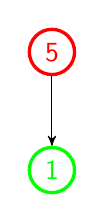
\begin{tikzpicture}[->,>=stealth',level/.style={sibling distance = 5cm/#1,
  level distance = 1.5cm}] 
\node [arn_r] {5}
	child{ node [arn_n] {1} 
    }
; 
\end{tikzpicture}
\\\\\large{Schritt 3:}
\\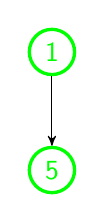
\begin{tikzpicture}[->,>=stealth',level/.style={sibling distance = 5cm/#1,
  level distance = 1.5cm}] 
\node [arn_n] {1}
	child{ node [arn_n] {5} 
    }
; 
\end{tikzpicture}
\\\\\large{Schritt 4:}
 \\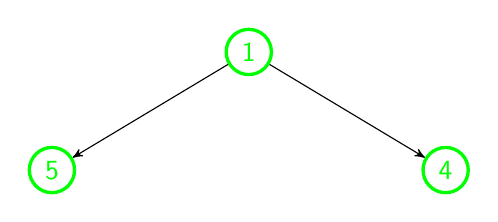
\begin{tikzpicture}[->,>=stealth',level/.style={sibling distance = 5cm/#1,
  level distance = 1.5cm}] 
\node [arn_n] {1}
	child{ node [arn_n] {5} 
    }
    child{ node [arn_n] {4}
    }
; 
\end{tikzpicture}
\\\\\large{Schritt 5:}
\\\\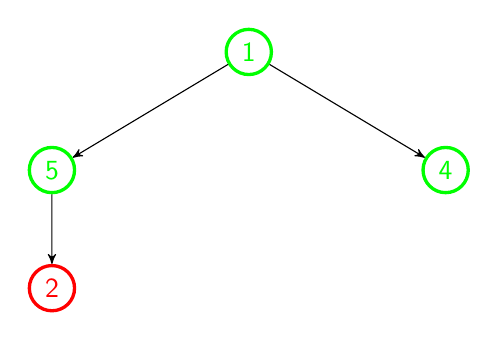
\begin{tikzpicture}[->,>=stealth',level/.style={sibling distance = 5cm/#1,
  level distance = 1.5cm}] 
\node [arn_n] {1}
	child{ node [arn_n] {5} 
		child{ node [arn_r] {2}}
    }
    child{ node [arn_n] {4}
    }
; 
\end{tikzpicture}
\\\\\large{Schritt 6:}
\\\\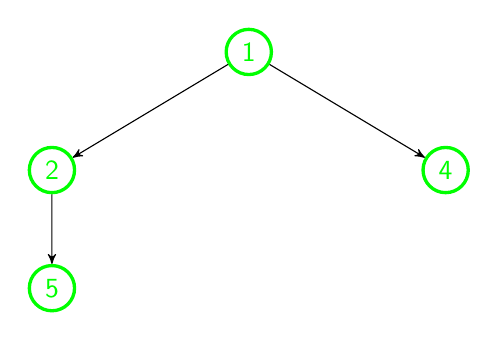
\begin{tikzpicture}[->,>=stealth',level/.style={sibling distance = 5cm/#1,
  level distance = 1.5cm}] 
\node [arn_n] {1}
	child{ node [arn_n] {2} 
		child{ node [arn_n] {5}}
    }
    child{ node [arn_n] {4}
    }
; 
\end{tikzpicture}
\end{minipage}
\begin{minipage}{7cm}
\large{Schritt 7:}
\\\\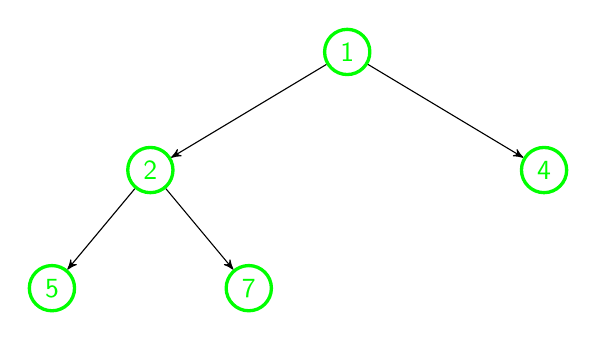
\begin{tikzpicture}[->,>=stealth',level/.style={sibling distance = 5cm/#1,
  level distance = 1.5cm}] 
\node [arn_n] {1}
	child{ node [arn_n] {2} 
		child{ node [arn_n] {5}}
			child{ node [arn_n] {7}}
    }
    child{ node [arn_n] {4}
    }
; 
\end{tikzpicture}
\\\\\large{Schritt 8:}
\\\\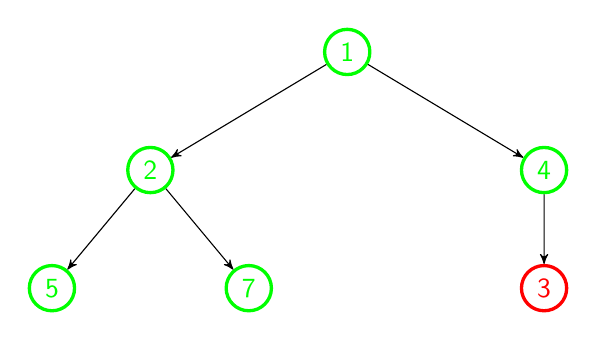
\begin{tikzpicture}[->,>=stealth',level/.style={sibling distance = 5cm/#1,
  level distance = 1.5cm}] 
\node [arn_n] {1}
	child{ node [arn_n] {2} 
		child{ node [arn_n] {5}}
			child{ node [arn_n] {7}}
    }
    child{ node [arn_n] {4}
    	child{ node[arn_r] {3}}
    }
; 
\end{tikzpicture}
\large{Schritt 9:}
\\\\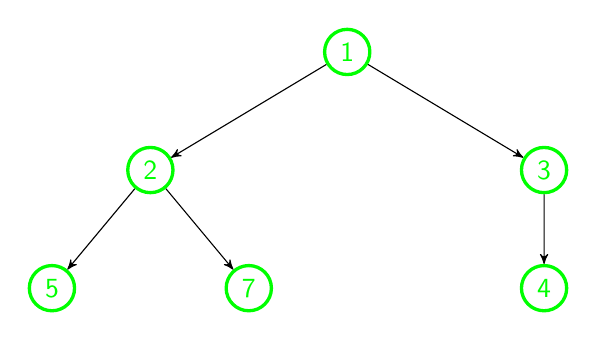
\begin{tikzpicture}[->,>=stealth',level/.style={sibling distance = 5cm/#1,
  level distance = 1.5cm}] 
\node [arn_n] {1}
	child{ node [arn_n] {2} 
		child{ node [arn_n] {5}}
			child{ node [arn_n] {7}}
    }
    child{ node [arn_n] {3}
    	child{ node[arn_n] {4}}
    }
; 
\end{tikzpicture}
\\\\\large{Schritt 10:}
\\\\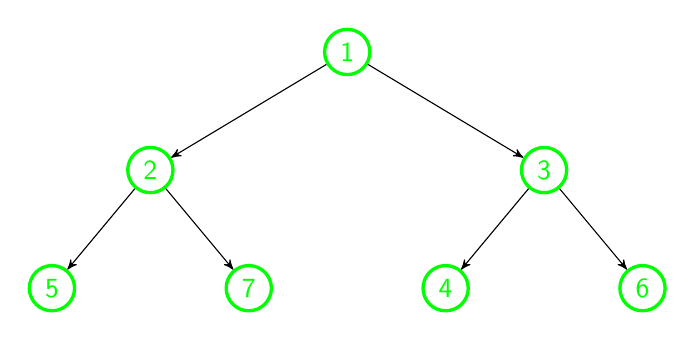
\begin{tikzpicture}[->,>=stealth',level/.style={sibling distance = 5cm/#1,
  level distance = 1.5cm}] 
\node [arn_n] {1}
	child{ node [arn_n] {2} 
		child{ node [arn_n] {5}}
			child{ node [arn_n] {7}}
    }
    child{ node [arn_n] {3}
    	child{ node[arn_n] {4}}
    		child{ node [arn_n] {6}}
    }
; 
\end{tikzpicture}
\end{minipage}
\end{flushleft}
%%%%%%%%% Sortieren
\pagebreak \large{Nun geht es ans Sortieren! Zuerst wird das Wurzelelement entfernt und in eine Liste geschrieben. Daraufhin wird das letzte Element des Heaps, also die 6 in Schritt 12 an die Stelle der Wurzel gesetzt. Nun ist die Heapbedingung verletzt und die 6 wird mit dem kleinsten der Kinder des Wurzelelements getauscht, also der 2 (Schritt 13). Die Heapbedingung ist nach wie vor verletzt und deshalb wird die 5 mit der 6 getauscht (Schritt 14). Nun ist der Heap wieder richtig und es geht weiter. Nun wird die neue Wurzel, also die 2 aus dem Heap entfernt und an die Liste angefügt, in der bereits die 1 steht. Nun wird in Schritt 15 das letzte Element, also die 4 an die Stelle der Wurzel eingefügt. Nun ist wieder die Heapbedingung verletzt. Daraufhin wird in Schritt 16 die 4 mit der 3 getauscht und der Heap ist wieder richtig. Nun wird das Neue Wurzelelement, also die 3, aus dem Heap entfernt und in die Liste gefügt und das letzte Element des Heaps, also die 7, an die Position der Wurzel geschrieben (Schritt 17). Nun ist die Heapbedingung wieder verletzt und es muss mit dem kleinsten Kind getauscht werden. Demnach wird in Schritt 18 die 7 mit der 4 getauscht und der Heap ist wieder richtig. Nun wird die 4 aus dem Heap entfernt und die 6 an die Position der Wurzel geschrieben (Schritt 19). Erneut ist die Heapbedingung verletzt und muss durch Tauschen mit dem kleinsten Kind wiederhergestellt werden. EWs wird demnach mit der 5 getauscht (Schritt 20). Es wird die 5 aus dem Heap entfernt und in die Liste geschrieben und das letzte Element des Heaps, also die 7, an die Position der Wurzel gesetzt (Schritt 21). Da die Heapbedingung weider verletzt ist, muss erneut getauscht werden. Denmach wird die 7 mit der 6 getauscht (Schritt 22) und der Heap ist wieder richtig. Zum Schluss enthält der Heap nur noch die 7, die dann auch entfernt und in die Liste geschrieben wird. Danach hat man eine sortierte Liste und einen leeren Heap. }
\begin{flushleft}
\begin{minipage}{7cm}
\large{Schritt 11:}
\\\\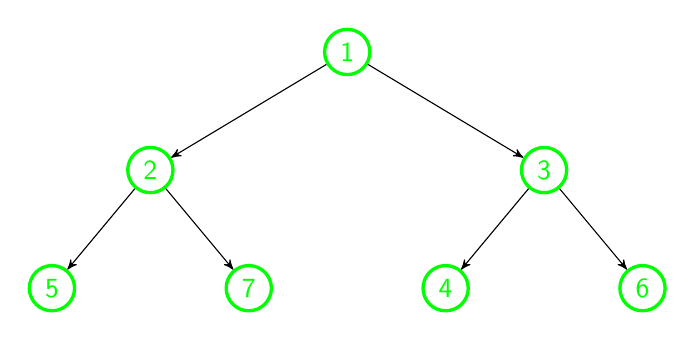
\begin{tikzpicture}[->,>=stealth',level/.style={sibling distance = 5cm/#1,
  level distance = 1.5cm}] 
\node [arn_n] {1}
	child{ node [arn_n] {2} 
		child{ node [arn_n] {5}}
			child{ node [arn_n] {7}}
    }
    child{ node [arn_n] {3}
    	child{ node[arn_n] {4}}
    		child{ node [arn_n] {6}}
    }
; 
\end{tikzpicture}
\\\\\large{Schritt 12:}
\\\\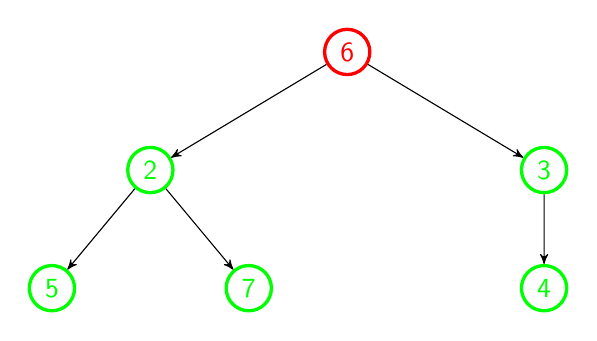
\begin{tikzpicture}[->,>=stealth',level/.style={sibling distance = 5cm/#1,
  level distance = 1.5cm}] 
\node [arn_r] {6}
	child{ node [arn_n] {2} 
		child{ node [arn_n] {5}}
			child{ node [arn_n] {7}}
    }
    child{ node [arn_n] {3}
    	child{ node[arn_n] {4}}
    }
; 
\end{tikzpicture}
\\\\\large{Schritt 13:}
\\\\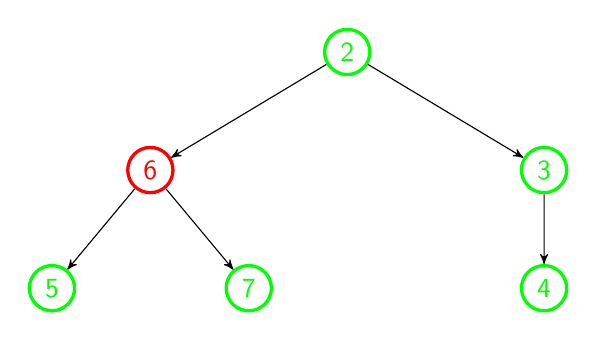
\begin{tikzpicture}[->,>=stealth',level/.style={sibling distance = 5cm/#1,
  level distance = 1.5cm}] 
\node [arn_n] {2}
	child{ node [arn_r] {6} 
		child{ node [arn_n] {5}}
			child{ node [arn_n] {7}}
    }
    child{ node [arn_n] {3}
    	child{ node[arn_n] {4}}
    }
; 
\end{tikzpicture}
\\\\\large{Schritt 14:}
\\\\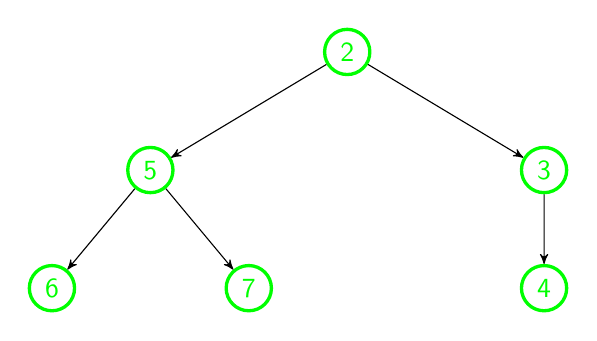
\begin{tikzpicture}[->,>=stealth',level/.style={sibling distance = 5cm/#1,
  level distance = 1.5cm}] 
\node [arn_n] {2}
	child{ node [arn_n] {5} 
		child{ node [arn_n] {6}}
			child{ node [arn_n] {7}}
    }
    child{ node [arn_n] {3}
    	child{ node[arn_n] {4}}
    }
; 
\end{tikzpicture}
\end{minipage}\hspace*{15mm}
\begin{minipage}{7cm}
\large{Schritt 15:}
\\\\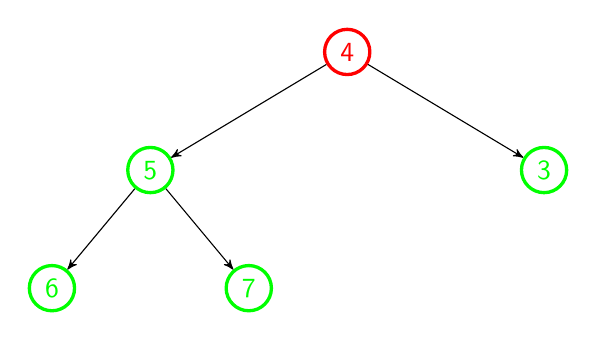
\begin{tikzpicture}[->,>=stealth',level/.style={sibling distance = 5cm/#1,
  level distance = 1.5cm}] 
\node [arn_r] {4}
	child{ node [arn_n] {5} 
		child{ node [arn_n] {6}}
			child{ node [arn_n] {7}}
    }
    child{ node [arn_n] {3}
    }
; 
\end{tikzpicture}
\\\\\large{Schritt 16:}
\\\\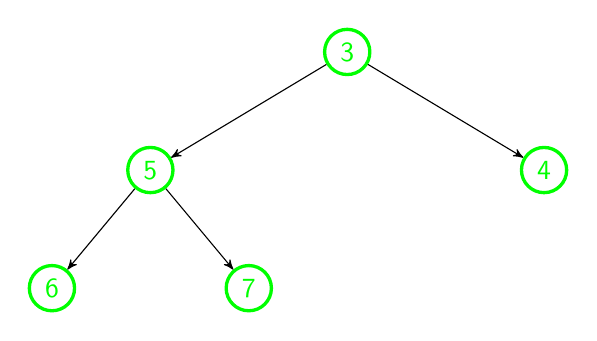
\begin{tikzpicture}[->,>=stealth',level/.style={sibling distance = 5cm/#1,
  level distance = 1.5cm}] 
\node [arn_n] {3}
	child{ node [arn_n] {5} 
		child{ node [arn_n] {6}}
			child{ node [arn_n] {7}}
    }
    child{ node [arn_n] {4}
    }
; 
\end{tikzpicture}
\\\\\large{Schritt 17:}
\\\\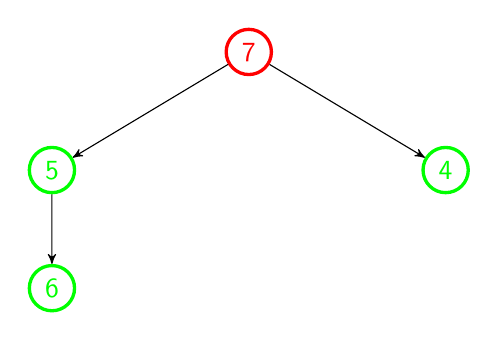
\begin{tikzpicture}[->,>=stealth',level/.style={sibling distance = 5cm/#1,
  level distance = 1.5cm}] 
\node [arn_r] {7}
	child{ node [arn_n] {5} 
		child{ node [arn_n] {6}}
    }
    child{ node [arn_n] {4}
    }
; 
\end{tikzpicture}
\\\\\large{Schritt 18:}
\\\\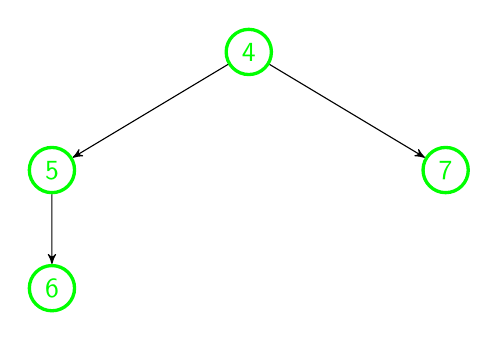
\begin{tikzpicture}[->,>=stealth',level/.style={sibling distance = 5cm/#1,
  level distance = 1.5cm}] 
\node [arn_n] {4}
	child{ node [arn_n] {5} 
		child{ node [arn_n] {6}}
    }
    child{ node [arn_n] {7}
    }
; 
\end{tikzpicture}
\end{minipage}
\end{flushleft}
\begin{flushleft}
\begin{minipage}{7cm}
\large{Schritt 19:}
\\\\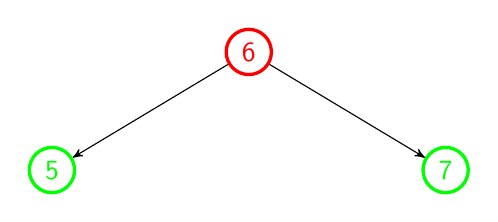
\begin{tikzpicture}[->,>=stealth',level/.style={sibling distance = 5cm/#1,
  level distance = 1.5cm}] 
\node [arn_r] {6}
	child{ node [arn_n] {5} 
    }
    child{ node [arn_n] {7}
    }
; 
\end{tikzpicture}
\\\\\large{Schritt 20:}
\\\\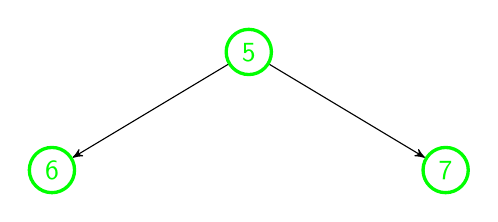
\begin{tikzpicture}[->,>=stealth',level/.style={sibling distance = 5cm/#1,
  level distance = 1.5cm}] 
\node [arn_n] {5}
	child{ node [arn_n] {6} 
    }
    child{ node [arn_n] {7}
    }
; 
\end{tikzpicture}
\end{minipage}\hspace*{15mm}
\begin{minipage}{7cm}
\large{Schritt 21:}
\\\\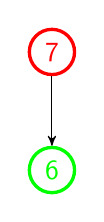
\begin{tikzpicture}[->,>=stealth',level/.style={sibling distance = 5cm/#1,
  level distance = 1.5cm}] 
\node [arn_r] {7}
	child{ node [arn_n] {6} 
    }
; 
\end{tikzpicture}
\\\\\large{Schritt 22:}
\\\\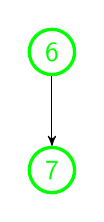
\begin{tikzpicture}[->,>=stealth',level/.style={sibling distance = 5cm/#1,
  level distance = 1.5cm}] 
\node [arn_n] {6}
	child{ node [arn_n] {7} 
    }
; 
\end{tikzpicture}
\end{minipage}
\end{flushleft}
\large{Schritt 23:}
\\\\
\begin{tikzpicture}[->,>=stealth',level/.style={sibling distance = 5cm/#1,
  level distance = 1.5cm}] 
\node [arn_n] {7}
; 
\end{tikzpicture}
\end{document}